\documentclass{beamer}
\mode<presentation>
\usetheme{CambridgeUS}
\usepackage[russian]{babel}
\usepackage[utf8]{inputenc}
\usepackage[T2A]{fontenc}
\usepackage{sansmathaccent}

\usepackage{verbatim}
\usepackage{alltt}

\pdfmapfile{+sansmathaccent.map}
\title[СУБД]{Процедурные расширения языка SQL}
\author{Наумов Д.А., доц. каф. КТ}
\date[29.03.2021] {Базы знаний и базы данных, 2021}

\begin{document}

%ТИТУЛЬНЫЙ СЛАЙД
\begin{frame}
  \titlepage
\end{frame}
  
%СОДЕРЖАНИЕ ЛЕКЦИИ
\begin{frame}
  \frametitle{Содержание лекции}
  \tableofcontents  
\end{frame}
  
%РАЗДЕЛ 1
\section{Основные понятия}
\begin{frame}
	\begin{itemize}
		\item База данных (БД) — совместно используемый набор логически связанных данных (и описание этих данных)
		\item База данных — совокупность данных, хранимых в соответствии со схемой данных, манипулирование которыми выполняют в соответствии с правилами средств моделирования данных 
		\item База данных — совокупность данных, организованных в соответствии с концептуальной структурой, описывающей характеристики этих данных и взаимоотношения между ними.
	\end{itemize}
\end{frame} 

\begin{frame}
	\begin{block}{Реляционная БД}
		база данных, основанная на реляционной модели данных.
	\end{block}
	РМД содержит следующие компоненты:
	\begin{itemize}
		\item Структура – данные в БД представляют собой набор отношений (relation) 
		\item Целостность – данные отвечают определенным условиям целостности
		\item Обработка – данные можно обрабатывать при помощи операторов манипулирования отношениями
	\end{itemize}
\end{frame} 

\begin{frame}
	\begin{center}
		\includegraphics[scale=0.4]{images/dbms.png}
	\end{center}
\end{frame} 

\begin{frame}{Основные объекты СУБД}
	\begin{itemize}
		\item Таблицы – фиксированное число столбцов, переменное число строк
		\item Индексы – служебные структуры для ускорения поиска
		\item Представления (view) – именованный запрос к таблицам
		\item Хранимые процедуры – именованная последовательность операторов
		\item Функции – процедуры, возвращающие значение (cкалярные, табличные)
		\item Триггеры – возможность обработки событий
		\item Пользователи – различные виды авторизации
		\item Роли – группы пользователей с одинаковым уровнем доступа
	\end{itemize}
\end{frame} 

\begin{frame}
\begin{minipage}{0.4\textwidth}
  \begin{flushleft}
	\begin{center}
		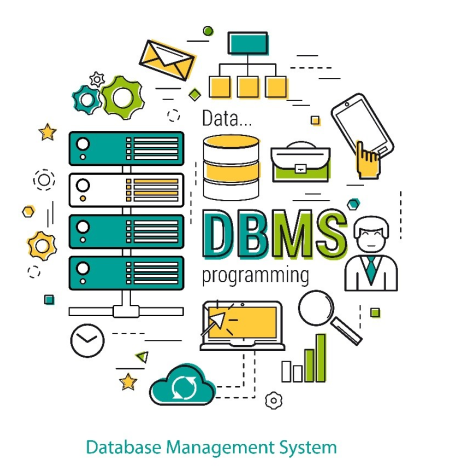
\includegraphics[scale=0.4]{images/DBMS-01.png}
	\end{center}
  \end{flushleft}
\end{minipage}
\begin{minipage}{0.4\textwidth}
  \begin{flushright}
  	\begin{itemize}
		\item Oracle Database
		\item Microsoft SQL Server
		\item MySQL (Oracle)
		\item IBM DB2
		\item IBM Informix
		\item SAP Sybase
		\item Teradata
		\item Firebird
		\item Microsoft Access
		\item PostgreSQL
  	\end{itemize}
  \end{flushright}
\end{minipage}
\end{frame}

\begin{frame}
\begin{minipage}{0.3\textwidth}
  \begin{flushleft}
	\begin{center}
		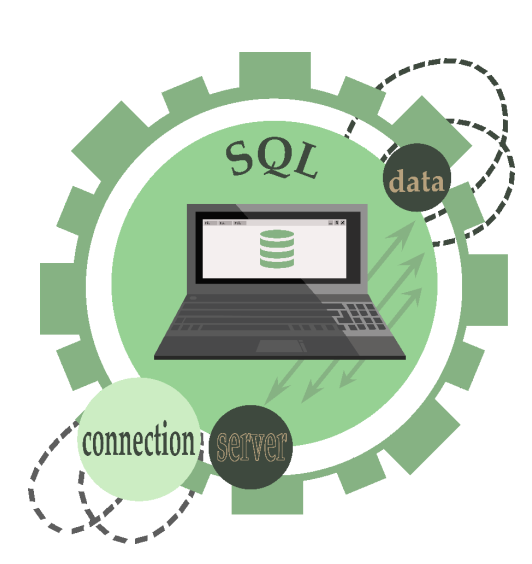
\includegraphics[scale=0.3]{images/SQL.png}
	\end{center}
  \end{flushleft}
\end{minipage}
\begin{minipage}{0.6\textwidth}
  \begin{flushright}
  	\begin{itemize}
		\item SQL – Structured Query Language
		\item Непроцедурный язык для работыс базами данных
		\item Первоначальное название – SEQUEL (Structured English Query Language)
		\item Создан в начале 1970-х годов, авторы – Дональд Чэмбэрлин (Donald D. Chamberlin) и Рэй Бойс (Ray Boyce)
		\item Первый стандарт: ANSI SQL-86, значительно доработан в 1992 (ANSI SQL-92)
		\item Последняя версия – SQL:2016 или ISO/IEC 9075:2016
  	\end{itemize}
  \end{flushright}
\end{minipage}
\end{frame}

\begin{frame}{Разделы SQL}
	Data Manipulation Language (DML) – язык манипулирования данными
	\begin{itemize}
		\item SELECT
		\item INSERT
		\item UPDATE
		\item DELETE
	\end{itemize}
	Transaction Control Language (TCL) – язык управления транзакциями
	\begin{itemize}
		\item BEGIN TRANSACTION / END TRANSACTION
		\item COMMIT / ROLLBACK
	\end{itemize}
	Data Definition Language (DDL) – язык описания данных
	\begin{itemize}
		\item CREATE TABLE, ALTER TABLE, TRUNCATE TABLE, DROP TABLE
		\item CREATE VIEW, ALTER VIEW, DROP VIEW
	\end{itemize}
	Data Control Language (DCL) – язык управления данными
	\begin{itemize}
		\item GRANT
		\item REVOKE
	\end{itemize}
\end{frame}

\begin{frame}{Типы данных MySQL}
	Символьные типы
	\begin{itemize}
		\item CHAR - строка фиксированной длины.
		\item VARCHAR - строка переменной длины.
		\item TINYTEXT: текст длиной до 255 байт.
		\item TEXT: представляет текст длиной до 65 КБ.
		\item MEDIUMTEXT: представляет текст длиной до 16 МБ
		\item LARGETEXT: представляет текст длиной до 4 ГБ
	\end{itemize}
	Типы для хранения двоичных данных
	\begin{itemize}
		\item TINYBLOB: данные длиной до 255 байт.
		\item BLOB: данные длиной до 65 КБ.
		\item MEDIUMBLOB: данные длиной до 16 МБ
		\item LARGEBLOB: данные длиной до 4 ГБ
	\end{itemize}
\end{frame}

\begin{frame}{Типы данных MySQL}
	Типы для работы с датой/временем
	\begin{itemize}
		\item DATE: хранит даты с 1 января 1000 года до 31 деабря 9999 года (c "1000-01-01" до "9999-12-31"). 
		\item TIME: хранит время от -838:59:59 до 838:59:59. 
		\item DATETIME: объединяет время и дату, диапазон дат и времени - с 1 января 1000 года по 31 декабря 9999 		года (с "1000-01-01 00:00:00" до "9999-12-31 23:59:59"). 
		\item TIMESTAMP: также хранит дату и время, в диапазоне: от "1970-01-01 00:00:01" UTC до "2038-01-19 03:14:07" UTC. 
		\item YEAR: хранит год в виде 4 цифр. 
	\end{itemize}
\end{frame}

\begin{frame}{Типы данных MySQL}
	Числовые типы данных
	\begin{itemize}
		\item TINYINT: целые числа от -127 до 128, 
		\item BOOL: TINYINT(1) 
		\item SMALLINT:  целые числа от -32768 до 32767
		\item MEDIUMINT: целые числа от -8388608 до 8388607
		\item INT: целые числа от -2147483648 до 2147483647
		\item BIGINT: целые числа от -9 223 372 036 854 775 808 до 9 223 372 036 854 775 807
		\item DECIMAL: числа с фиксированной точностью DECIMAL(precision, scale).
		\item FLOAT: числа с плавающей точкой одинарной точности
		\item DOUBLE: числа с плавающей точкой двойной точности 
	\end{itemize}
\end{frame}

\begin{frame}{NULL-значения}
	\begin{minipage}{0.3\textwidth}
		\begin{flushleft}
			\begin{center}
				
\includegraphics[scale=0.3]{images/NULL.png}
			\end{center}
		\end{flushleft}
	\end{minipage}
	\begin{minipage}{0.6\textwidth}
		\begin{flushright}
			\begin{itemize}
				\item NULL – ключевое слово SQL, обозначающее отсутствие данных
				\item Не следует путать значение NULL со значением по умолчанию для какого-либо столбца или типа данных
				\item Любая арифметическая или логическая операция с NULL приводит к NULL
				\item NULL добавляет в SQL элементы троичной логики
				\item Для обработки значения NULL предусмотрены специальные функции и операторы языка SQL
			\end{itemize}
		\end{flushright}
	\end{minipage}
\end{frame}

\begin{frame}{Клиент и сервер}
	\begin{minipage}{0.3\textwidth}
		\begin{flushleft}
			\begin{center}
				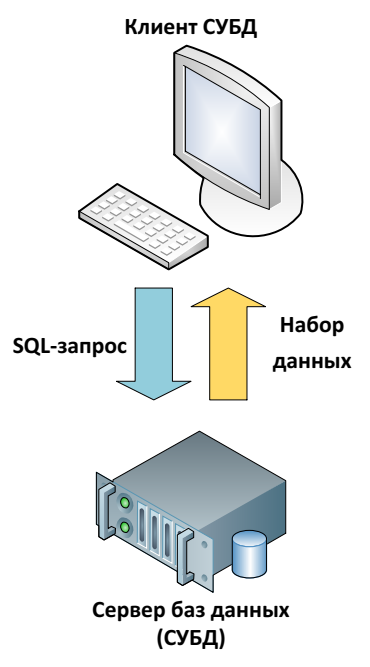
\includegraphics[scale=0.3]{images/Server.png}
			\end{center}
		\end{flushleft}
	\end{minipage}
	\begin{minipage}{0.6\textwidth}
		\begin{flushright}
			\begin{itemize}
				\item Клиент и сервер обмениваются данными c использованием определенного программного протокола: ODBC, OLEDB, JDBC, собственный (native) клиент
				\item Все, что может послать клиент SQL-серверу – это SQL-запрос
				\item Все, что может послать в ответ SQL-сервер клиенту – набор данных или текстовое сообщение о какой-либо ошибке
				\item Набор данных – это таблица 
				\item В предельном случае таблица может содержать ровно один столбец и ровно одну строку 						\end{itemize}
		\end{flushright}
	\end{minipage}
\end{frame}

\begin{frame}{Структура оператора SELECT}
	\begin{center}
		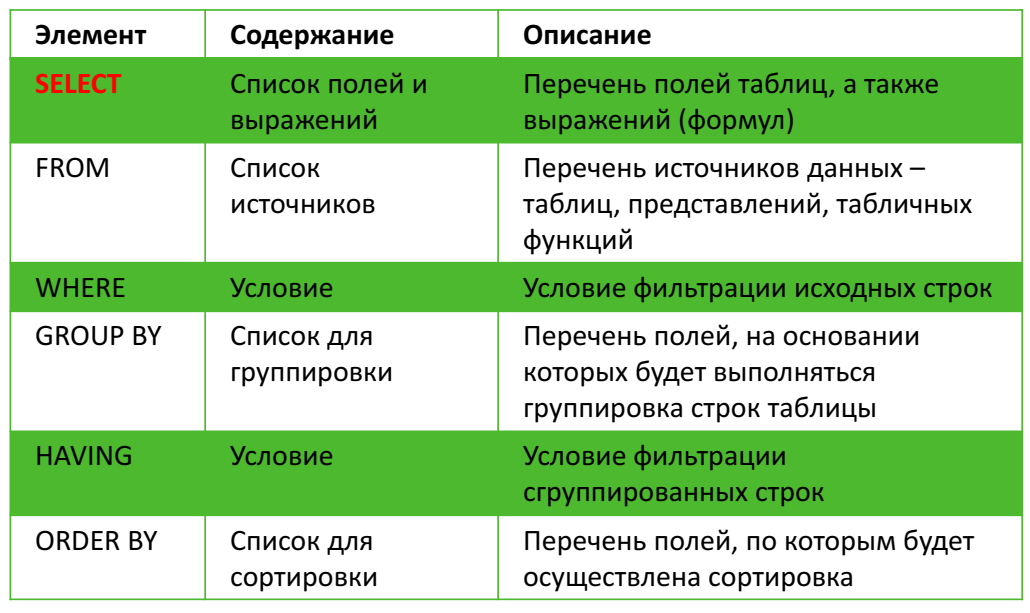
\includegraphics[scale=0.4]{images/Select-01.png}
	\end{center}
\end{frame}

\begin{frame}{Простейший оператор SELECT}
	\begin{minipage}{0.3\textwidth}
		\begin{flushleft}
			\begin{itemize}
				\item SELECT 1
				\item SELECT 2*2, 3*3
				\item SELECT CURDATE() AS Today
				\item SELECT '1' + '3'
		  	\end{itemize}
			\begin{center}
				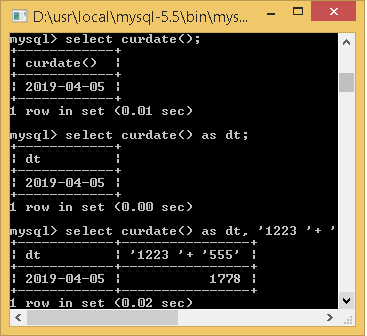
\includegraphics[scale=0.2]{images/SQL-01.png}
			\end{center}
		\end{flushleft}
	\end{minipage}
	\begin{minipage}{0.6\textwidth}
		\begin{flushright}
			\begin{itemize}
				\item Простейший оператор SELECT не содержит даже элемента FROM 
				\item Он содержит перечень констант или выражений, включая вызовы скалярных функций
				\item Для назначения именам столбцов используется ключевое слово AS, но оно является необязательным. Тем не менее, рекомендуется его использовать – это делает запрос более читаемым 
				\item Математические операторы: +, –, *, / 
				\item Конкатенация строк: CONCAT(,)
			\end{itemize}
		\end{flushright}
	\end{minipage}
\end{frame}

\begin{frame}{Выборка данных из таблицы}
	\begin{minipage}{0.4\textwidth}
		\begin{flushleft}
			\begin{center}
				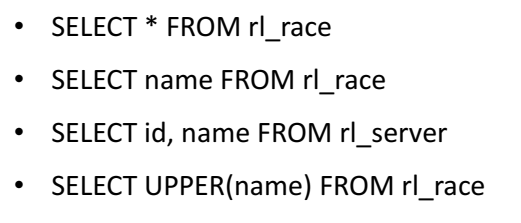
\includegraphics[scale=0.4]{images/SQL-01a.png}
		  	\end{center}
			\begin{center}
				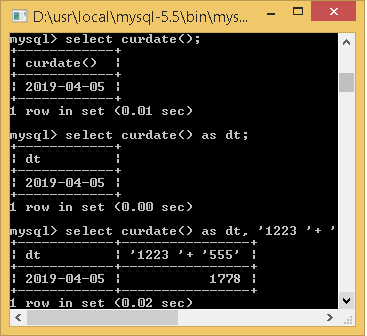
\includegraphics[scale=0.2]{images/SQL-01.png}
		  	\end{center}
	  	\end{flushleft}  	
	\end{minipage}
	\begin{minipage}{0.5\textwidth}
		\begin{flushright}
			\begin{itemize}
				\item Элемент FROM задает таблицу, из которой необходимо извлечь данные
				\item Звездочка (*) означает "все столбцы"
				\item Использование звездочки в реальных запросах крайне не рекомендуется
				\item Столбцы таблицы перечисляются через запятую
				\item Возможно использование скалярных функций
				\item Порядок строк в возвращаемом наборе данных не определен и не может быть гарантирован без дополнительных указаний
			\end{itemize}
		\end{flushright}
	\end{minipage}
\end{frame}

\begin{frame}
	\begin{center}
		\includegraphics[scale=0.4]{images/sql-02.png}
	\end{center}
\end{frame} 

\begin{frame}
	\begin{center}
		\includegraphics[scale=0.5]{images/sql-03.png}
	\end{center}
\end{frame} 

\begin{frame}
	\begin{center}
		\includegraphics[scale=0.5]{images/sql-04.png}
	\end{center}
\end{frame} 

\begin{frame}{Условные вычисления}
	\begin{minipage}{0.4\textwidth}
		\begin{flushleft}	
			\begin{center}
				\includegraphics[scale=0.5]{images/sql-05.png}
			\end{center}
		\end{flushleft}  	
	\end{minipage}
	\begin{minipage}{0.5\textwidth}
		\begin{flushright}
			\begin{itemize}
				\item При необходимости можно осуществлять условные вычисления непосредственно в тексте запроса
				\item Для этого, например, может быть использована встроенная функция IF, имеющая три аргумента
				\item Первый аргумент – логическое выражение 
				\item IF возвращает значение второго аргумента, если логическое выражение истинно
				\item IF возвращает значение третьего аргумента, если логическое выражение истинно
			\end{itemize}
		\end{flushright}
	\end{minipage}
\end{frame}

\begin{frame}
	\begin{center}
		\includegraphics[scale=0.5]{images/sql-06.png}
	\end{center}
\end{frame} 

\begin{frame}
	\begin{center}
		\includegraphics[scale=0.5]{images/cs-01.png}
	\end{center}
\end{frame} 

\begin{frame}
	\begin{center}
		\includegraphics[scale=0.5]{images/cs-02.png}
	\end{center}
\end{frame} 

\begin{frame}
	\begin{center}
		\includegraphics[scale=0.5]{images/cs-03.png}
	\end{center}
\end{frame} 

\begin{frame}
	\begin{center}
		\includegraphics[scale=0.5]{images/cs-04.png}
	\end{center}
\end{frame} 

\begin{frame}
	\begin{center}
		\includegraphics[scale=0.5]{images/cs-05.png}
	\end{center}
\end{frame} 

\begin{frame}
	\begin{center}
		\includegraphics[scale=0.5]{images/cs-06.png}
	\end{center}
\end{frame} 

\begin{frame}
	\begin{center}
		\includegraphics[scale=0.5]{images/union.png}
	\end{center}
\end{frame} 

\begin{frame}
	\begin{center}
		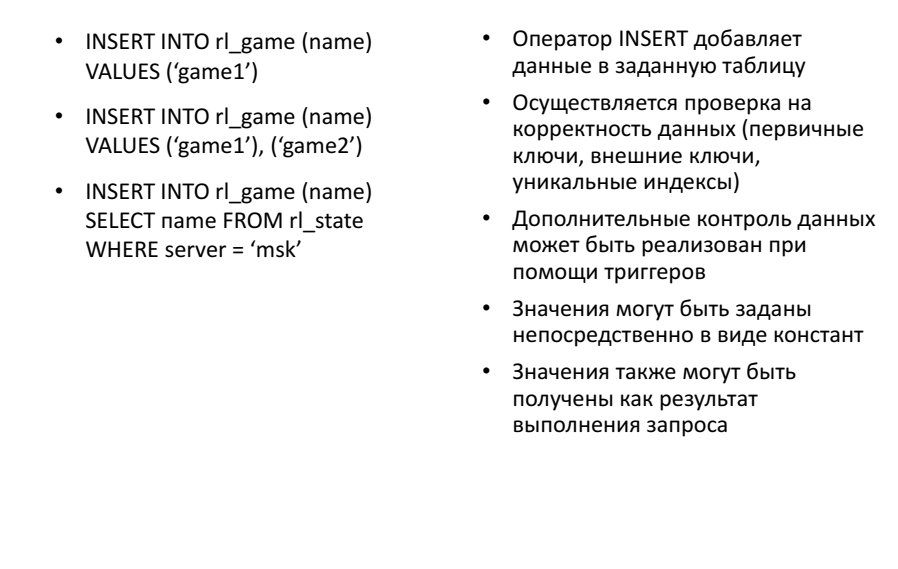
\includegraphics[scale=0.5]{images/insert-01.png}
	\end{center}
\end{frame} 

\begin{frame}
	\begin{center}
		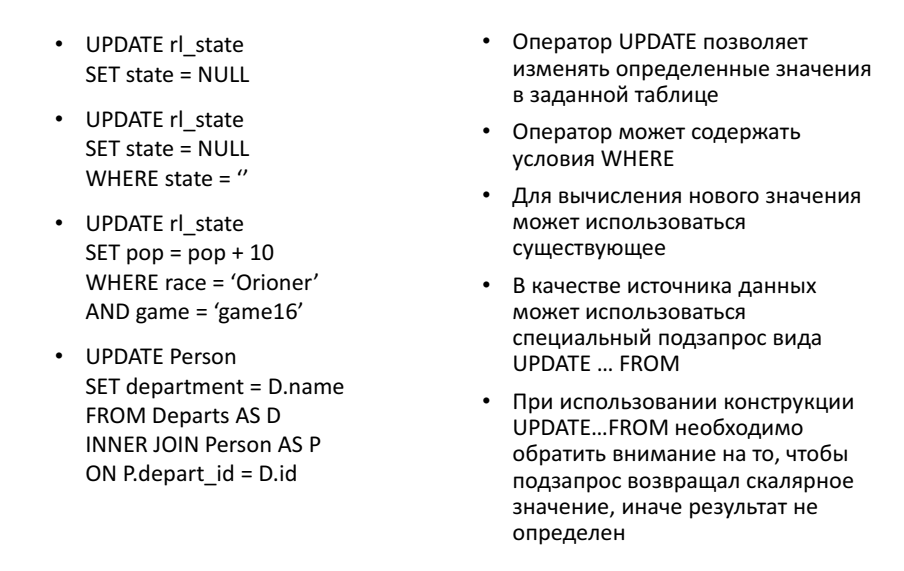
\includegraphics[scale=0.5]{images/update-01.png}
	\end{center}
\end{frame} 

\begin{frame}
	\begin{center}
		\includegraphics[scale=0.5]{images/delete-01.png}
	\end{center}
\end{frame} 

\begin{frame}
	\begin{center}
		\includegraphics[scale=0.5]{images/group.png}
	\end{center}
\end{frame} 

\begin{frame}
	\begin{center}
		\includegraphics[scale=0.5]{images/avg.png}
	\end{center}
\end{frame} 

\begin{frame}
	\begin{center}
		\includegraphics[scale=0.5]{images/having.png}
	\end{center}
\end{frame} 

\end{document}